% The original template (from Trevor) had a custom \appendix command,
% but I found it to break figure/table counters. I'm not sure how
% reliable my fix is, so I ended up reverting back to the standard
% latex version, and renaming the custom command to \myappendix.  You
% can try both and see how things work out:
% 1) Call \appendix once, and then make each appendix a \chapter
% 2) Call \myappendix once, and then make each appendix a \section.

%\appendix
\chapter{Example Figures}

% Appendix sections, subsections etc should not appear in the table of 
% contents. So set tocdepth to 0 and set it back to 2 at the end. Do 
% this for each appendix.
\addtocontents{toc}{\protect\setcounter{tocdepth}{0}}

%%%%%%%%%%%%%%%%%%%%%%%%%%%%%%%%%%%%%%%%%%%%%%%%%%%%%%%%%%%%%%%%%%%%%%%%%
% Example Normal Figure                                                 %
%%%%%%%%%%%%%%%%%%%%%%%%%%%%%%%%%%%%%%%%%%%%%%%%%%%%%%%%%%%%%%%%%%%%%%%%%
\begin{figure}
    \centering
    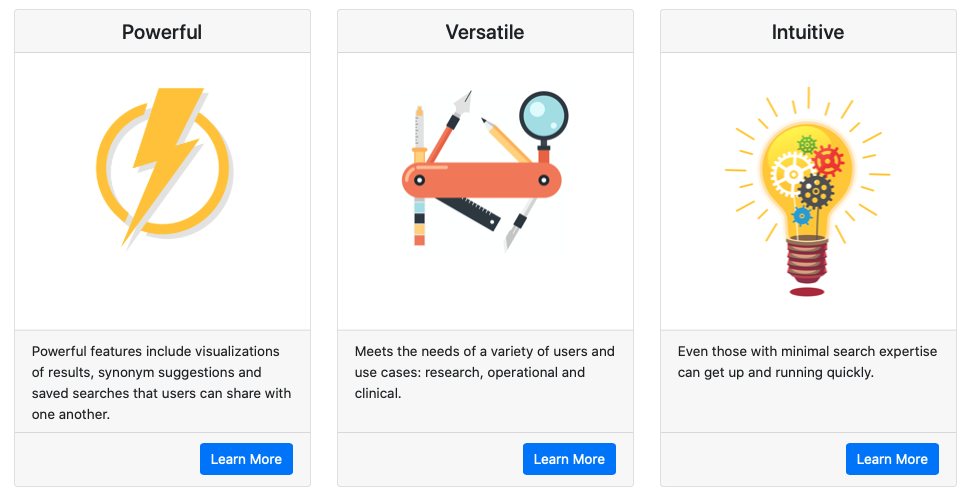
\includegraphics[width=0.8\textwidth]{Resources/Images/Banner4.png}
    \caption{Caption}
    \label{fig:my_label}
\end{figure}

%%%%%%%%%%%%%%%%%%%%%%%%%%%%%%%%%%%%%%%%%%%%%%%%%%%%%%%%%%%%%%%%%%%%%%%%%
% Example Sub-Figure with Sub-Captions                                  %
%%%%%%%%%%%%%%%%%%%%%%%%%%%%%%%%%%%%%%%%%%%%%%%%%%%%%%%%%%%%%%%%%%%%%%%%%
\begin{figure}
    \centering
    \begin{subfigure}{0.4\textwidth}
        
\includegraphics[width=\textwidth]{Resources/Images/Banner1.png}
        \caption[width=\textwidth]{Example Image 1}
        \label{fig:sub_bigrams3_apdx}
    \end{subfigure}
    \hfill
    \begin{subfigure}{0.4\textwidth}
        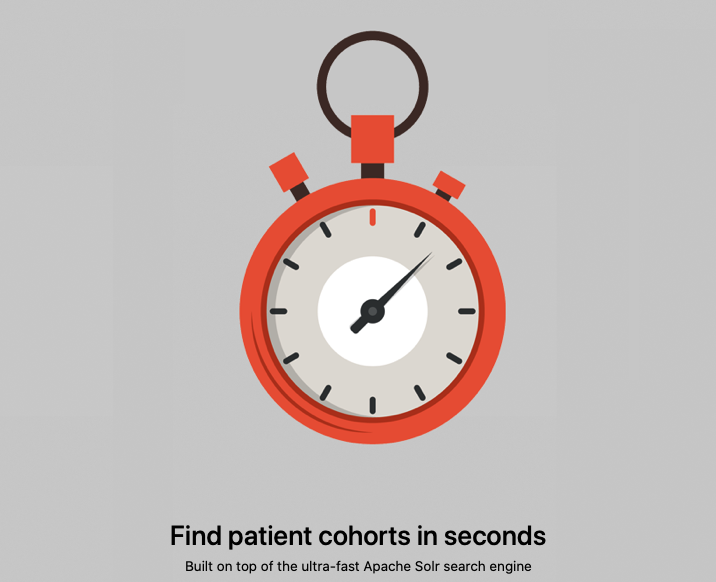
\includegraphics[width=\textwidth]{Resources/Images/Banner2.png}
        \caption[width=\textwidth]{Example Image 2}
        \label{fig:sub_trigrams3_apdx}
    \end{subfigure}
    \hfill
    \caption{Example multi-image figure}
    \label{fig:subfig_example}
\end{figure}

%%%%%%%%%%%%%%%%%%%%%%%%%%%%%%%%%%%%%%%%%%%%%%%%%%%%%%%%%%%%%%%%%%%%%%%%%
% Example Figure with Wrapped Text                                      %
%%%%%%%%%%%%%%%%%%%%%%%%%%%%%%%%%%%%%%%%%%%%%%%%%%%%%%%%%%%%%%%%%%%%%%%%%
\begin{wrapfigure}{L}{0.5\textwidth}
    \centering
    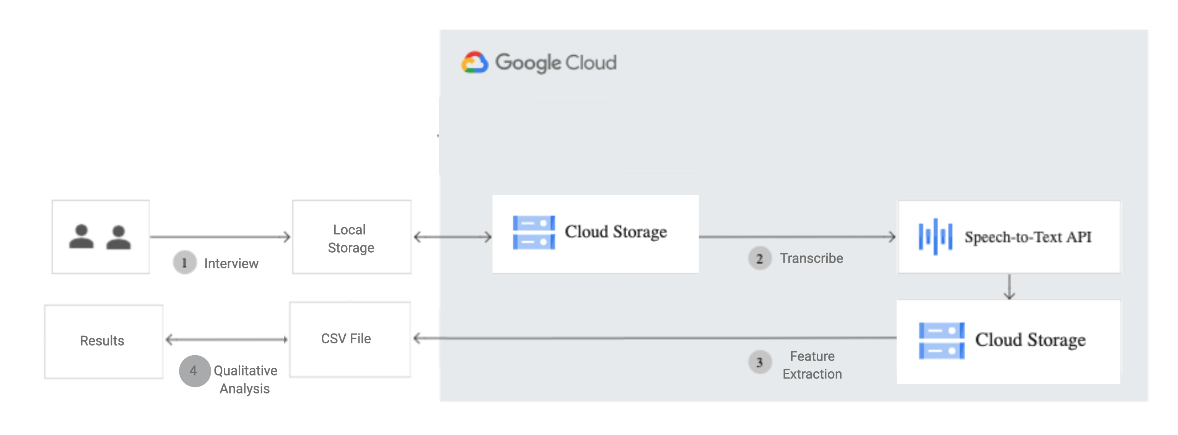
\includegraphics[width=0.45\textwidth]{Resources/Images/Workflow2.png}
    \caption{Example of figure that text will wrap around}
    \label{fig:UM_interview_wordcloud}
\end{wrapfigure}
\lipsum[1]
\lipsum[2]


\addtocontents{toc}{\protect\setcounter{tocdepth}{2}}